\usepackage{nccmath}

\showtocfalse

\begin{document}

%----------------------------------------------------------------------------------------
%	TITLE PAGE
%----------------------------------------------------------------------------------------

\title[FL - Signal Processing Perspective]{Federated Learning \\ {\smaller[2] A Signal Processing Perspective}}
\date{}
\author[]{}

% \institute[北京航空航天大学] % Your institution as it will appear on the bottom of every slide, may be shorthand to save space
% {
% 数学科学学院 \\ % Your institution for the title page
% \medskip
% \textit{wenh06@gmail.com} % Your email address
% 北京航空航天大学 \\
% 数学科学学院 \qquad 北京航空航天大学
% }

% \logo{\includegraphics[height=1.5cm]{logo}}
% \logoii{\includegraphics[height=1cm]{logo2}}

% \date{\footnotesize 2021年4月13日} % Date, can be changed to a custom date

\setlength{\belowdisplayskip}{5pt} \setlength{\belowdisplayshortskip}{5pt}
\setlength{\abovedisplayskip}{5pt} \setlength{\abovedisplayshortskip}{5pt}

%------------------------------------------------

\begin{frame}
\titlepage % Print the title page as the first slide
\end{frame}

%------------------------------------------------
% Page 1

\begin{frame}
\frametitle{Main Problems}

\begin{block}{Scenario}
{\color{red}Wireless} cross-device
\end{block}

\vspace{1em}

\begin{block}{Main Problems}
\begin{figure}
\centering
\begin{tikzpicture}
\node[] at (0, 0) (theta) {$\theta_t^i$};
\node[] at (2, 0) (s) {\color{red}$s_t^i$};
\node[] at (4, 0) (x) {\color{red}$x_t^i$};
\node[] at (6, 0) (y) {\color{red}$y_t$};
\node[] at (8, 0) (global) {$\theta_t$};
\path [draw, -Stealth] (theta) -- node [midway,above,align=center] {\smaller encode} (s);
\path [draw, -Stealth] (s) -- node [midway,above,align=center] {\smaller transmit} (x);
\path [draw, -Stealth] (x) -- node [midway,above,align=center] {\smaller aggregate} (y);
\path [draw, -Stealth] (y) -- node [midway,above,align=center] {\smaller combine} (global);
\node[below = 0em of theta] (lm) {local model};
\node[below = 0em of global] (gm) {global model};
\end{tikzpicture}
\end{figure}
\end{block}

\blfootnote{\tiny \cite{Gafni_2022}\bibentry{Gafni_2022}}

\end{frame}

%------------------------------------------------

\section{Encode}

%------------------------------------------------
% Page 1

\begin{frame}
\frametitle{Encode}

$$\text{encoded model} \to s_t^i = \phi_i(\theta_t^i)$$

\begin{block}{Purpose and Methods}
\begin{itemize}
\item Compression
  \begin{itemize}
      \item sparsification
      \item quantization
      \item $\cdots$
  \end{itemize}
\item Privacy
  \begin{itemize}
      \item multi-party encryption (computation, MPC)
      \item homomorphic encryption (HE)
      \item differential privacy (DP)
      \item $\cdots$
  \end{itemize}
\end{itemize}
\end{block}

\end{frame}

%------------------------------------------------

\section{Transmission \& Aggregation}

%------------------------------------------------
% Page 1

\begin{frame}
\frametitle{Transmission}

{\color{red} Wireless scenario}
$$\text{channel input} \rightarrow x_t^i = \varphi_i(s_t^i \leftarrow \text{encoded model})$$

\vspace{1em}

\begin{block}{Key Points}
\begin{itemize}
\item Learning-Aware Resource Allocation
\item Over-the-Air Federated Learning (AirFL)
\end{itemize}
\end{block}

\end{frame}

%------------------------------------------------
% Page 1

\begin{frame}
\frametitle{Learning-Aware Resource Allocation}

\begin{block}{User Selection \& {\color{red} Resource Management}}
{\smaller
{\color{red}\noindent RM: relevant only for users that communicate over the same media \\
$\to$ each user having a separate channel with the server.
}
}
\begin{itemize}
\item Random selection
\item Delay Minimization With Probabilistic User Selection
  \begin{itemize}
      \item Probabilistic User Selection
      \vspace{-0.5em}
      {\smaller
      $$\rho_t^i = \alpha_t \dfrac{\lVert \theta_t^i - \theta_{t-E}^i \rVert}{\sum\limits_{i=1}^N \lVert \theta_t^i - \theta_{t-E}^i \rVert} + (1-\alpha_t)\dfrac{\max_j d_j - d_i}{N\max_j d_j - \sum\limits_{i=1}^N d_i}$$
      }
      \vspace{-0.7em}
      \item Delay-Minimizing Resource Division
      \vspace{-1em}
      {\smaller
        $$
        \min_{\{\chi_{t,k}^i\}_{k=1}^K \in \{0, 1\}^K} \max_{i\in\mathcal{G}_t} \dfrac{\beta_t^i}{\sum\limits_{k=1}^K \chi_{t,k}^i R_{i,k}} \quad
        \text{s.t.} \sum\limits_{i\in\mathcal{G}_t} \chi_{t,k}^i = \sum\limits_{k=1}^K \chi_{t,k}^i = 1
        $$
        }
  \end{itemize}
  \vspace{-0.7em}
  {\smaller \color{red}
  $d$: distance to the access point; $\beta$: model size (bits); $R$: data rate over the channel.
  }
\end{itemize}
\end{block}

\end{frame}

%------------------------------------------------
% Page 1

\begin{frame}
\frametitle{Over-the-Air Federated Learning (AirFL)}

Users simultaneously employ the complete temporal and spectral resources (complete reuse) of the uplink channel in a nonorthogonal manner.
\vspace{-1em}
\begin{figure}
\centering
\begin{tikzpicture}
\node[] at (0, 0) (aircomp) {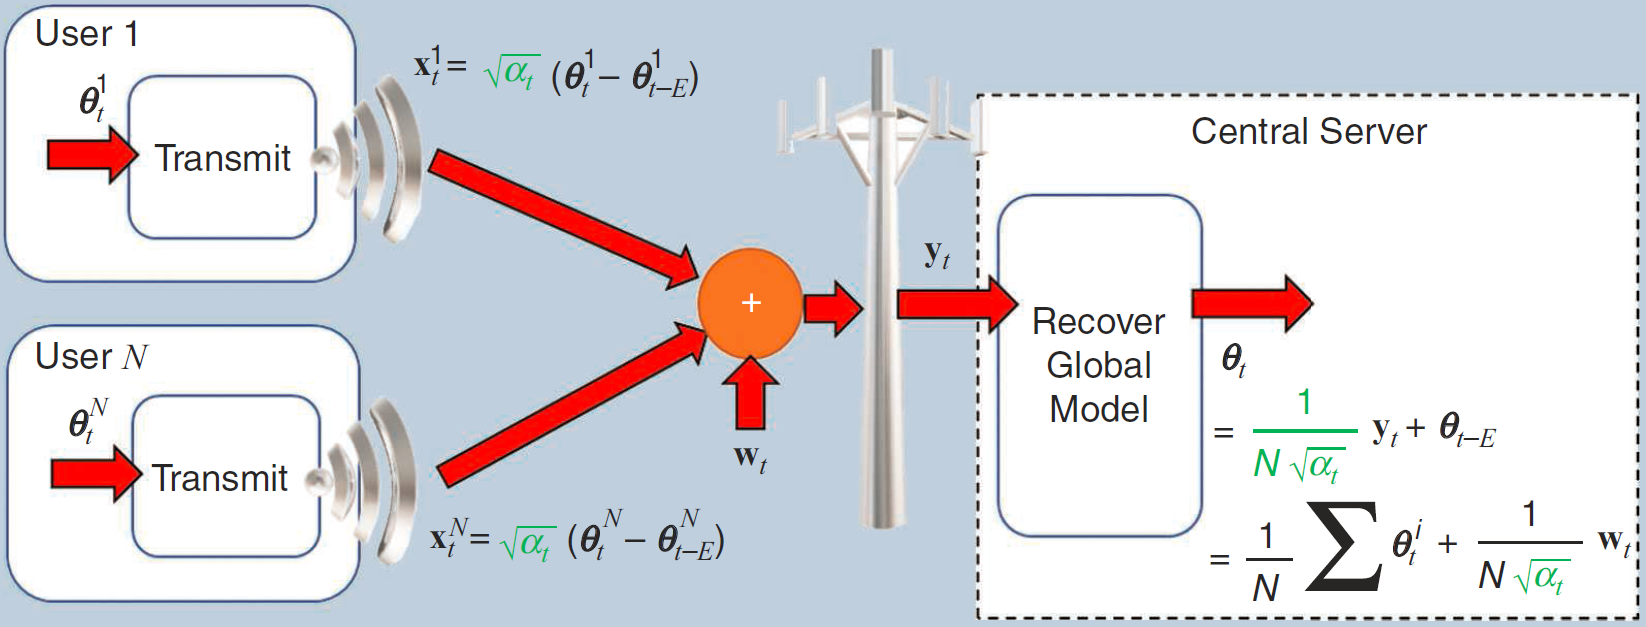
\includegraphics[width=\textwidth]{images/AirFL.png}};
\node[text centered] at (2.5,1.8) (cs) {\smaller\color{red}Compressed Sensing};
\node[] at (1.5,1.5) (mimo) {\smaller\color{red}MIMO};
\path[color=red, thick, -Stealth] ([yshift = 0.2em]mimo.west) edge (0.5,1.3);
\end{tikzpicture}
\end{figure}

Flat fading channel with Gaussian noise and {\color{cyan}interference}:
$$y^i_t = h^ix^i_t + w^i_t {\color{cyan} + v_k}$$

\end{frame}

%------------------------------------------------
% Page 1

\begin{frame}
\frametitle{Analog Aggregation-Based FL\cite{Fan_2021_AirFL}}

{\smaller
\begin{align*}
y_t & = \sum p_t^i \odot x_t^i \odot h_t^i + w_t \\
(p_t^i)_d & = \dfrac{(\beta_t^i)_d K_i (b_t)_d}{(h_t^i)_d} ~~ \text{power control vector}
\end{align*}
}

\begin{block}{Optimization Problem}
\begin{figure}
\centering
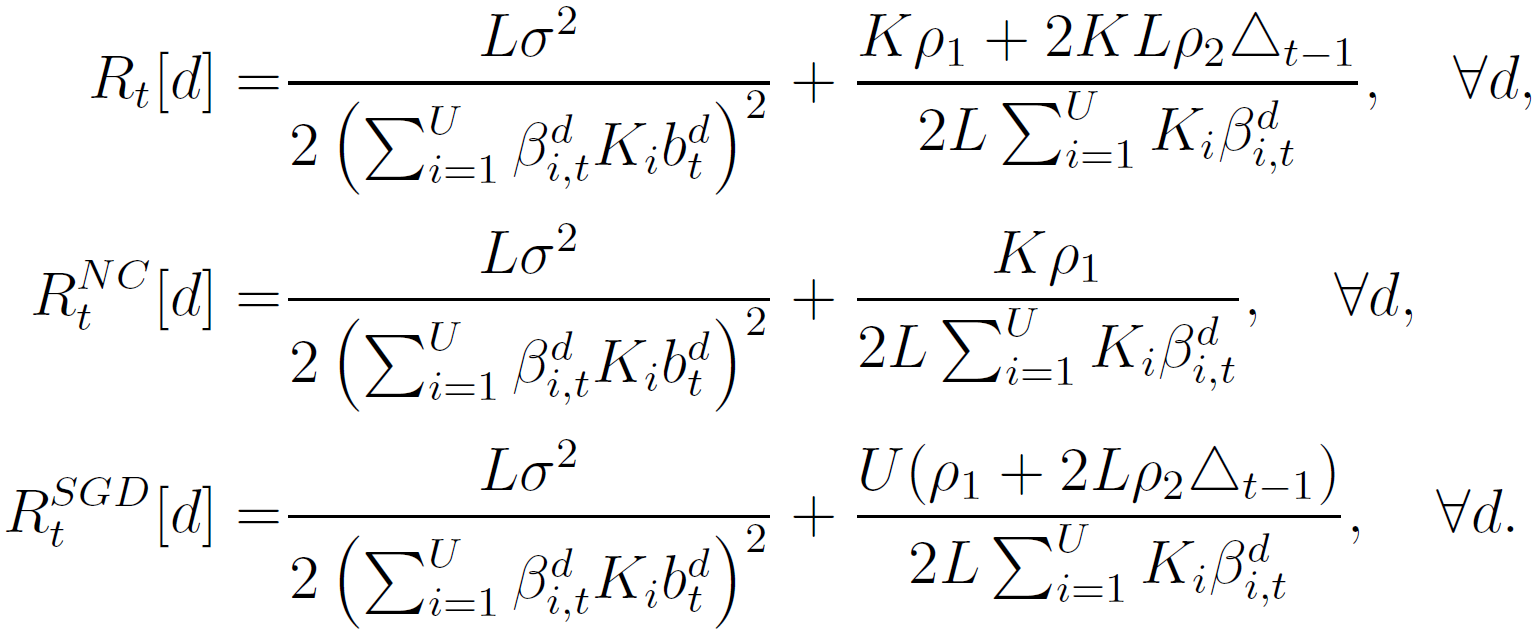
\includegraphics[width=0.46\textwidth]{images/AirFL-objective.png}
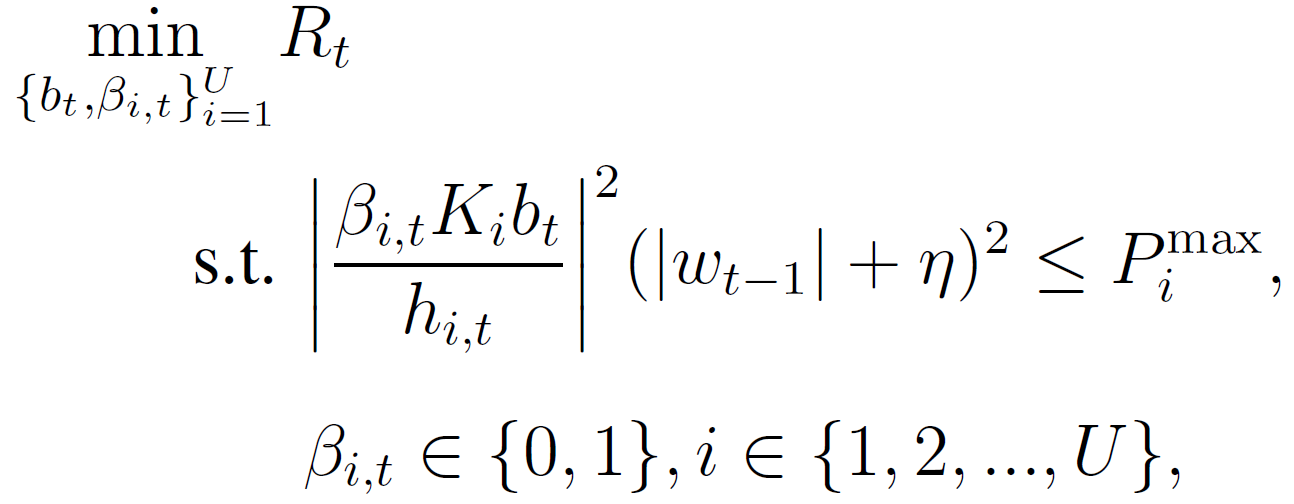
\includegraphics[width=0.49\textwidth]{images/AirFL-P3.png}
\end{figure}
\end{block}

\blfootnote{\tiny \cite{Fan_2021_AirFL}\bibentry{Fan_2021_AirFL}}

\end{frame}

%------------------------------------------------
% Page 1

\begin{frame}
\frametitle{AirComp\cite{Liu_2020_AirComp}}

\begin{figure}
\centering
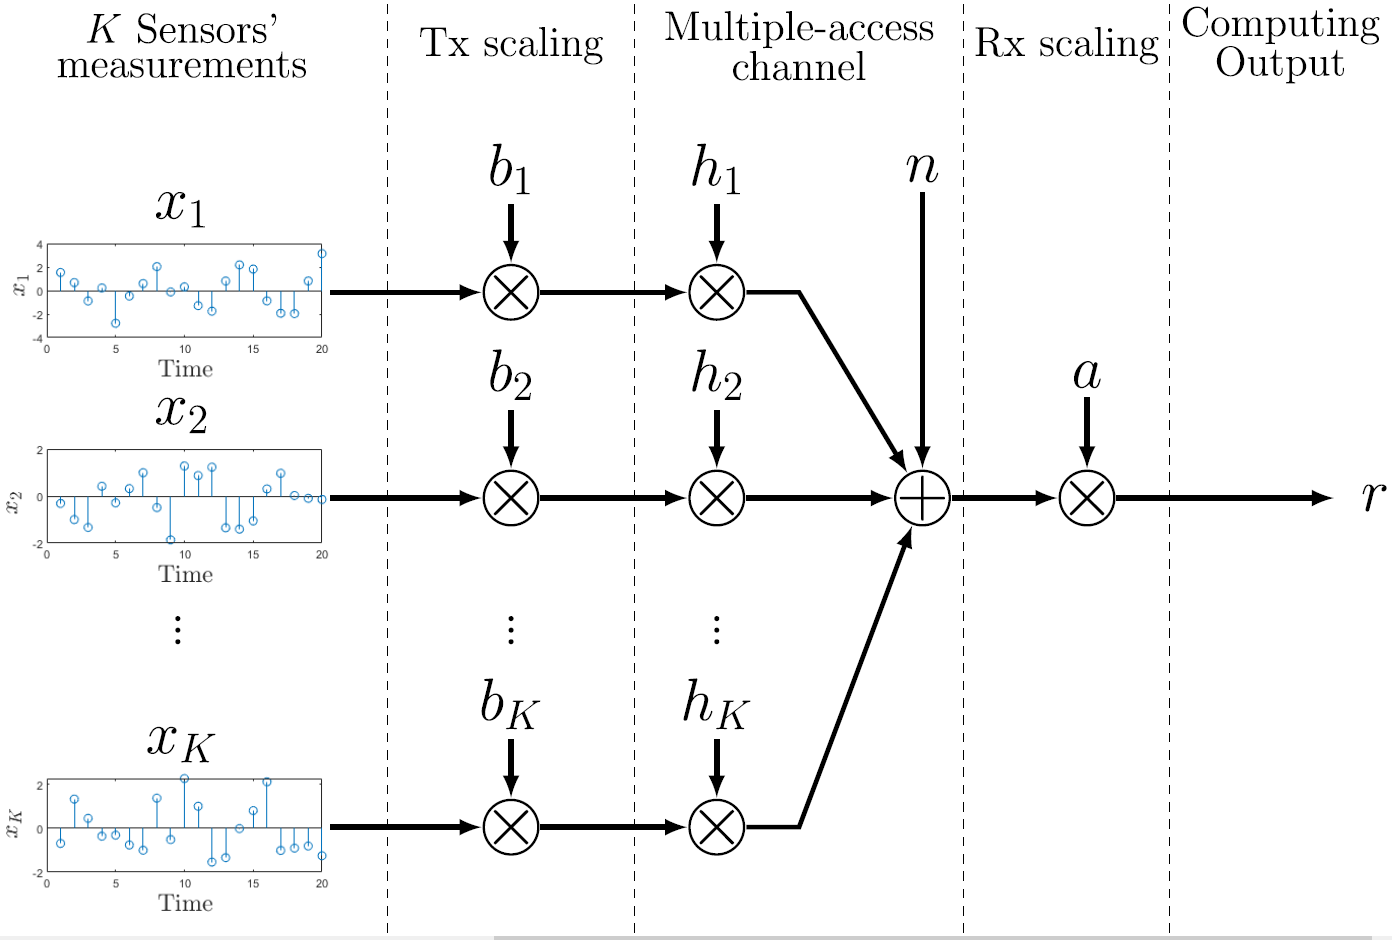
\includegraphics[width=0.8\textwidth]{images/AirComp.png}
\end{figure}

\blfootnote{\tiny \cite{Liu_2020_AirComp}\bibentry{Liu_2020_AirComp}}

\end{frame}

%------------------------------------------------
% Page 1

\begin{frame}
\frametitle{Time-Varying Precoding for AirFL}

\begin{align*}
y_t & = \sum\limits_{i=1}^N x^i_t + w_t, ~~ x^i_t = \sqrt{\alpha_t}(\theta_t^i - \theta_{t-E}^i) \\
\theta_t & = \dfrac{1}{\sqrt{\alpha_t}} y_t + \theta_{t-E} = \dfrac{1}{N} \sum\limits_{i=1}^N \theta_t^i + \dfrac{1}{N\sqrt{\alpha_t}} w_t \\
{\color{red}\alpha_t\ } & {\color{red}= \dfrac{P}{\max_i \mathbb{E}\{\lVert \theta_t^i - \theta_{t-E}^i \rVert\}}}
\end{align*}

\begin{figure}
\centering
\begin{tikzpicture}
\node[] at (0, 0) (theta) {$\theta_t^i$};
\node[] at (2, 0) (s) {\color{red}$s_t^i$};
\node[] at (4, 0) (x) {\color{red}$x_t^i$};
\node[] at (6, 0) (y) {\color{red}$y_t$};
\node[] at (8, 0) (global) {$\theta_t$};
\path [draw, -Stealth] (theta) -- node [midway,above,align=center] {\smaller encode} (s);
\path [draw, -Stealth] (s) -- node [midway,above,align=center] {\smaller transmit} (x);
\path [draw, -Stealth] (x) -- node [midway,above,align=center] {\smaller aggregate} (y);
\path [draw, -Stealth] (y) -- node [midway,above,align=center] {\smaller combine} (global);
\node[below = 0em of theta] (lm) {local model};
\node[below = 0em of global] (gm) {global model};
\end{tikzpicture}
\end{figure}

\end{frame}

%------------------------------------------------
% Page 1

\section{Combining}

%------------------------------------------------
% Page 1

\begin{frame}
\frametitle{Combining}

\begin{block}{Mixture of models}
\begin{figure}
\centering
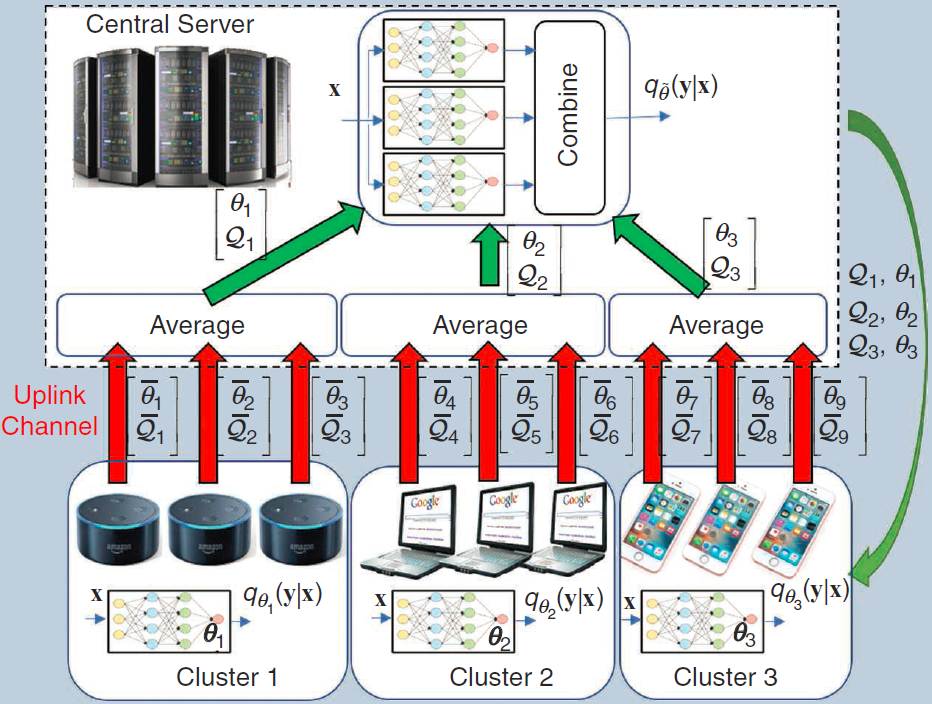
\includegraphics[width=0.75\textwidth]{images/mixture-models.png}
\end{figure}
\end{block}

\end{frame}

%------------------------------------------------
% Page 1

\begin{frame}
\frametitle{Combining}

\begin{block}{Security: Byzantine–Robust Combining}
\begin{itemize}
    \item Geometric median combining:
    \vspace{-0.5em}
    {\smaller
    $$\theta_t = \argmin_{\theta} \sum \lVert \theta - y_t^i \rVert_2$$}
    \vspace{-1em}
    \item Krum aggregation\cite{NIPS2017_krum}:
    \vspace{-0.5em}
    {\smaller
    \begin{align*}
    & \theta_t = KR(y_1,\ldots,y_N) = y_{i_*}, ~~ i_* = \argmin_{i} \sum\limits_{i\to j} \lVert y_i - y_j \rVert^2 \\
    & i\to j: \text{the set of $N-f-2$ nearest neighbors.}
    \end{align*}}
    \vspace{-2em}
    \item Truncation mapping: discards ``abnormal'' subset of the model updates before averaging.
\end{itemize}
\end{block}

\blfootnote{\tiny \cite{NIPS2017_krum}\bibentry{NIPS2017_krum}}

\end{frame}

%------------------------------------------------
% Page 1

\begin{frame}[allowframebreaks]
\frametitle{References}

{\footnotesize
\bibliographystyle{ieeetr}
\bibliography{references}
}

\end{frame}

%------------------------------------------------

\end{document}
